\section{Framework}\label{sec:framework}
%\textbf{MANCA UNA INTRO MOTIVANTE DELLO SCHEMA}\\
%Considering the aforementioned requirements, we designed the conceptual framework that employed conducting perceptual experiments. We identify the following entities that are in relation to each other in numerous ways. 
In this Section, we introduce a framework for the design of perceptual experiments on musical performances. The framework is composed of five main entities, which interact with each other in numerous ways, depending on the kind of experiment we want to conduct and performance we aim to observe. The framework can be considered as a first formalization of the problem of investigating NMP, and we aim to develop it further during the project.

We show in Figure \ref{fig:framework} a schematic representation of the framework and the basic relations among entities. A \textbf{performance} occurs when two or more \textbf{subjects} musically interact together through a \textbf{medium}. Subjects can be musicians during a rehearsal, as well as teachers and students. In order to consider a large number of probable scenarios, a performance can occur with all the subjects in the same room (\textit{local performance}), with all the subjects geographically distant (\textit{networked performance}) or with part of the subjects in the same place and part of the subjects geographically distant (\textit{mixed performance}). Subjects interact by means of a \textit{medium}. In the case of local performances, the medium is a \textit{physical medium}, such as simple air propagation. In the case of networked performances, the medium is \textit{networked medium}, such as an Internet connection and the NMP software/hardware equipment to connect the two subjects. In the case of mixed performance both physical medium and networked medium are involved. 

In all the scenarios subjects perform in an \textbf{environment} with specific timbral (acoustic of the room) and spatial properties (location of the subjects in the room). In the case of networked and mixed performance, environments with different characteristics are potentially involved. Given a subject, we define the environment he/she playing as the \textit{real environment} and the environment they perceive of the geographically-distant subjects as the \textit{virtual environment}. For example, in Figure \ref{fig:afsv}, we show a set of frames from one of the experiments we conducted. Fig. \ref{subfig:as} shows a harp player in her \textit{real} environment; her partner's perception of this environment, i.e., the \textit{virtual environment}, is shown in Fig. \ref{subfig:av}. 

%Since the investigation of the sense of presence is one of the main goals of the experiments, the study of the interaction between the real environment with the virtual environment is crucial. This 

%\textbf{DIRE QUALCOSA IN PIU\' DI QUALI ELEMENTI ENTRANO IN GIOCO}.

%the environments are different, the subjects will interact through a \textit{networked medium}, hence having a NMP; otherwise they interact through a \textit{physical medium}. The comparison between a networked and physical medium is crucial to understand how to design the interaction so that the \textit{virtual environment} perceived from the other end of the medium matches the expectations of a real environment. 

In order to analyze the performance, it is crucial to run a \textbf{data recording} stage, using different devices to capture the multimodal signals. The factors and aspects that will be possible to analyze from the performance depend on the properties of the devices, e.g., whether they are \textit{video} or \textit{audio devices}, or where they are placed. In the following sections we describe in detail the aforementioned entities.



\begin{figure}[t]
	\centering
	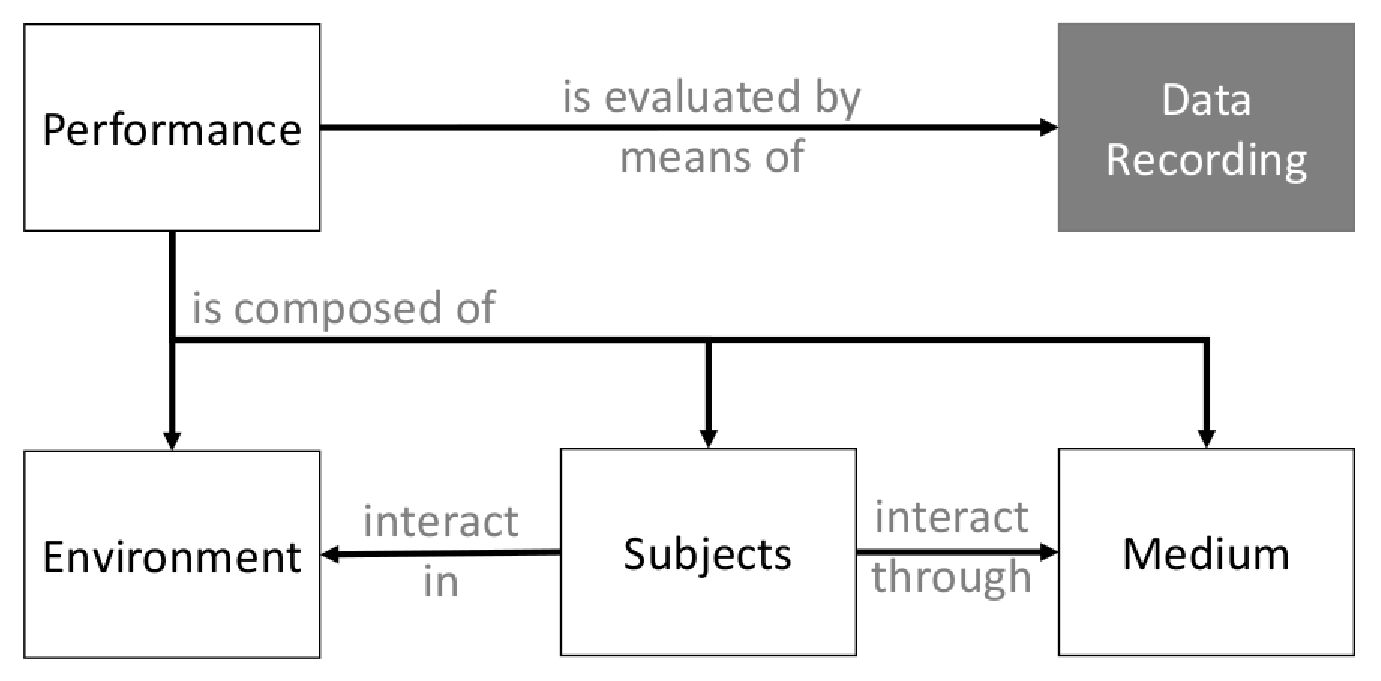
\includegraphics[width=\columnwidth]{img/framework.eps}
	\caption{A graphical representation of the proposed framework with main entities and interaction.}
	\label{fig:framework}
\end{figure}

\subsection{Performance}
In our experiments we consider two types of performances: \textit{performed piece} or \textit{taught lesson}. The performance is the entity at the highest hierarchical level and it is composed of the subjects, the environments and the mediums. 
Main properties of the performance are date and time, location(s), types of performance, such as is better detailed in the subjects' \textit{part} property, metadata (e.g., composer of the piece, tempo, meter, key signature, score, duration, etc.) and composition  description in form of symbolic representation (MIDI or musicXML) \cite{MIDItoolbox}.

Some properties of the performance depend on the nature of its sub-entities. For example, if the subjects are two musicians, the performance can be a \textit{rehearsal} or a \textit{concert}, while if one of the subject is a teacher, the performance is defined as a \textit{lesson}. As discussed above, the property of performance also depends on the type of medium: we have a networked or mixed performance if we have at least one networked medium.   

\subsection{Subjects}
Subjects are involved in the performance with different possible roles, such as musicians, students, teachers or conductors. Subjects are identified with their name, age, experience, musical background, that evolve over time and so must be referred to the day of the performance. Other properties inherently related to a subject is the assigned part -what they are performing- and the used instrument. These two properties can be also described by means of a content-based analysis of their musicological (e.g., rhythmic complexity) or timbral (e.g. attack time) properties, respectively \cite{RottondiFeature}.
Doing this, it is possible to analyze how such properties as aspects that may affect the final quality or success of the performance.


\subsection{Environment}
We refer to the spatial and acoustic properties of both the physical place where a subject performs and the perception of it by the other subjects as physical and virtual environment, respectively. The properties of the virtual environment depend on the location and specifics of the audio/video capture and rendering devices, such as the microphone and speakers connected to the NMP equipment. For example, using an array of microphones we can capture the acoustic scene~\cite{Markovic2013} and render it using arrays of speakers through spatial audio techniques~\cite{bianchi2016}.

Properties of the environment are also the possible processing applied to the audio or video signals. For example, by applying a reverb to the incoming audio signal, a subject will have a different perception of the virtual enviornment.

We also collect the information about the interaction of the subjects with the environment, such as the position of the musicians in the room, the details of the audio/video acquisition (e.g., microphone on the instrument vs. fixed position microphone) and the relative position of musician and devices. 

\subsection{Medium}
The medium refers to the connection between the environments and, hence, the subjects. In case of a networked performance, the medium collects the information on the employed software for NMP and its settings, the network architecture and specifics, like bandwidth, latency. In case of a performance in the same room, like a traditional lesson, we collect information as the distance between the subjects, which measures the acoustic latency between them, and describe possible visual / acoustic occlusion that may be placed between the musicians. 


\begin{table}
	\centering
	\caption{Details of the experiment in co-presence}
	\begin{tabular}{p{1.5cm}p{6cm}}
		\hline
		\textbf{Entity} & \textbf{Properties} \\
		\hline
		\textbf{Performance} & Co-presence performance. \newline Parts arranged from Bartok pieces as described in [cit]. \\
		\textbf{Subjects} & Two brothers, violin and cello players. \newline Violin player: male, 25 years, 17 years musical experience; 	\newline Cello player: male, 19 years, 10 years  musical experience \\
		\textbf{Environment} & Recording and mastering studio in the Conservatory of Milan; acoustically equipped with bass traps. \newline Musicians sit side by side, with peripherical vision.\\
		\textbf{Medium} & Condition 1: Air propagation. \newline Condition 2: Visual occlusion applied by means of a a screen with progressive layers of canvas applied to decrease transparency and visibility. \\
		\textbf{Data} \newline \textbf{recording}  & Interview to the participants and free comments.\\
		\hline
	\end{tabular}
	\label{tab:exp1}
\end{table}


\subsection{Data recording}
In order to observe the experiment and draw meaningful conclusions, we need to record the properties of the performance that are interesting for our analysis. For the data recording stage, we consider multimodal signals and their processing byproduct as well as questionnaire filled by the subjects. In the former case, we can extract objective metrics of the performance, while in the latter we consider subjective results; both are important to assess the outcome of the experiment. 

With regard to the multimodal signals, the audio recording of the performance, from the two environments, are clearly useful to assess the quality of the performance or possible modifications in the timbral or rhythmic properties. Beyond that, video recordings are also useful to annotate saccadic movement during the interaction between the subjects \cite{vandemoortele2018gazing}, and we aim to capture biometric signals to objectively estimate the subjective distress of the performers \cite{Yoshie2009}. 
